\subsection{Convertidor CC-CC Conmutado}

Para llevar a cabo el diseño del convertidor, primero debemos establecer los objetivos de rendimiento del mismo (como por ejemplo, la tensión que debe tener a la salida). Con estos valores establecidos, y junto con otras consideraciones del diseño, se van a obtener todos los parámetros que definen al convertidor, como las llaves y diodos a utilizar, tamaño de capacitores e inductores, etc.\\

\begin{figure}[h]
    \centering
    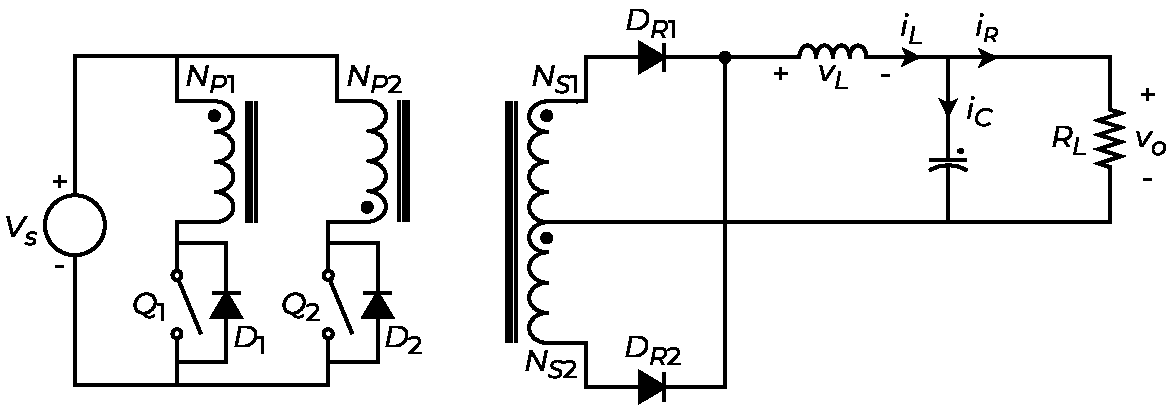
\includegraphics[scale=0.6]{Imagenes/Push-Pull.pdf}
    \caption{Diagrama del convertidor CC-CC de tipo puente completo a utilizar, con todos sus componentes (Placeholder).}
    \label{puente_completo}
\end{figure}

\subsubsection{Especificaciones de Diseño}

La plataforma experimental va a ser utilizada para la evaluación de un módulo de pilas de combustible de \SI[]{300}[]{\watt} de potencia nominal, entregando \SI[]{36}[]{\volt} a \SI[]{8.3}[]{\ampere} de corriente. La tensión de salida varía desde \SI[]{65}[]{\volt} a circuito abierto hasta \SI[]{30}[]{\volt} para la máxima corriente de \SI[]{9.5}[]{\ampere}.\textsuperscript{\cite{HSeriesBrochure}}\\

Esta potencia debe ser transferida por el convertidor hacia la carga variable a la salida, que emula distintas condiciones de carga del bus común de corriente continua de \SI[]{75}[]{\volt} fijos. Dada la potencia de \SI[]{300}[]{\watt}, y si la tensión de salida es la del bus común, entonces el sistema debe soportar una corriente de salida máxima de alrededor de \SI[]{4}[]{\ampere}. Adicionalmente, las llaves del primario van a conmutar a una frecuencia de conmutación de \SI[]{20}[]{\kilo\hertz}, y se debe reducir lo más posible las pérdidas de energía por conmutación, para darle una mayor escalabilidad al diseño.\\

\begin{itemize}
    \item {\SemiBold Potencia nominal \textit{P\textsubscript{N}}:}\quad\SI[]{300}[]{\watt}
    \item {\SemiBold Tensión de salida \textit{v\textsubscript{o}}:}\quad\SI[]{75}[]{\volt}
    \item {\SemiBold Corriente de salida \textit{i\textsubscript{o}}:}\quad\SI[]{4}[]{\ampere}
    \item {\SemiBold Tensión de entrada \textit{v\textsubscript{FC}}:}\quad\SI[]{65}[]{\volt}\textsubscript{máx} , \SI[]{30}[]{\volt}\textsubscript{mín}
    \item {\SemiBold Corriente de entrada \textit{i\textsubscript{FC}}:}\quad\SI[]{9.5}[]{\ampere}
    \item {\SemiBold Frecuencia de conmutación \textit{f\textsubscript{s}}:}\quad\SI[]{20}[]{\kilo\hertz}\\
\end{itemize}

Entonces, con todas estas características quedan definidas las especificaciones necesarias para comenzar la selección y dimensionamiento de componentes del convertidor. Se va a tratar el diseño de cada componente uno por uno, comenzando por los cuatro transistores de potencia que se encargan de la conmutación.\\

\subsubsection{Selección de Llaves}

Las cuatro llaves ideales que conforman el circuito puente del lado primario son implementadas por algún dispositivo electrónico de tres terminales (los polos positivo y negativo de la llave, y un tercer terminal de control con el que se comanda la conmutación de la llave). Existen dentro de estas llaves dos categorías distintas: las \textit{llaves semicontroladas}, donde la llave no se puede controlar completamente (por ejemplo se puede comandar el cierre pero no la apertura) y las \textit{llaves completamente controladas} que, como su nombre dice, pueden ser cerradas y abiertas mediante su tercer terminal.\\

En nuestro caso, la topología de puente completo exige la apertura y cierre de las cuatro llaves a la frecuencia de conmutación, por lo que se requieren {\Medium llaves completamente controladas}. Dentro de esta categoría existen tres tipos distintos de transistores de potencia que vamos a evaluar para utilizar en la plataforma: el transistor bipolar o BJT (\textit{Bipolar Junction Transistor}), el transistor IGBT (\textit{Insulated-Gate Bipolar Transistor}) y el transistor de efecto de campo o MOSFET (\textit{Metal-Oxide-Semiconductor Field-Effect Transistor}).\\

\paragraph{Transistor Bipolar}

\lipsum[1]\\

\paragraph{IGBT}

\lipsum[1]\\

\paragraph{MOSFET}

\lipsum[1]\\